%@TheDoctorRAB
%standard white paper/preproposal format
%
%%%%%
%
%REFERENCES
%
%neup.bst - numbered citations in order of appearance, short author list with et al in reference section
%nsf.bst - numbered citations in order of appearance, full author list in references section
%standard.bst - citations with author last name with et al for more than 2 authors; full author list in references section
%ans.bst is for ANS only. 
%
%author = {Lastname, Firstname and Lastname, Firstname and Lastname, Firstname} for all bst formats
%bst renders the author list itself
%
%author = {{Nuclear Regulatory Commission}} if the author is an organization, institution, etc., and not people
%
%title = {{}} for all
%
%for all - use \citep{-} - [1] or (Borrelli, 2021) in the text
%standard.bst \cite{-} - Borrelli (2021) in the text
%standard.bst lists references alphabetically
%the rest list numerically
%
%
%%% slides 
%
%\citep{xxxnna} where the citation should go
%\blfootnote{\fontsize\cite{xxxnna}\fontsize\bibentry{xxxnna}} before \end{frame}
%
%
%%%%%

%%%%% presentation settings
\documentclass[aspectratio=1610,pdftex,dvipsnames,compress,xcolor={dvipsnames}]{beamer}
\usetheme{Boadilla}
\usecolortheme{seahorse}
\beamertemplatenavigationsymbolsempty
\addtobeamertemplate{footnote}{\hskip -2em}{} %pushes footnote to margin
\setbeamerfont{title}{series=\bfseries}
\setbeamertemplate{page number in head/foot}[framenumber] %just gives slide number; comment out for 1/7, 2/7...
\definecolor{BackGround}{RGB}{255,250,240}
\setbeamercolor{background canvas}{bg=BackGround}
\setbeamertemplate{caption}[numbered]
%%%%%


%%%%% general 
%\documentclass[11pt,a4paper]{article}
%\usepackage[lmargin=1in,rmargin=1in,tmargin=1in,bmargin=1in]{geometry}
\usepackage[pagewise]{lineno} %line numbering
\usepackage{setspace}
\usepackage{ulem} %strikethrough - do not \sout{\cite{}}
\usepackage{graphicx}
\usepackage{mypythonhighlight,verbatim}
\usepackage{filecontents}
\usepackage{tablefootnote}
\usepackage{footnotehyper}
\usepackage{float}
%\usepackage{subfig}
\usepackage[yyyymmdd]{datetime} %date format
\renewcommand{\dateseparator}{.}
\graphicspath{{img/}} %path to graphics
\setcounter{secnumdepth}{5} %set subsection to nth level
\usepackage{needspace}
\usepackage[stable,hang,flushmargin]{footmisc} %footnotes in section titles and no indent; standard.bst
\usepackage[inline]{enumitem}
\setlist[itemize]{label=\textbullet}
\usepackage{boldline}
\usepackage{makecell}
\usepackage{booktabs}
\usepackage{amssymb}
\usepackage{gensymb}
\usepackage{amsmath,nicefrac}
\usepackage{physics}
\usepackage{lscape}
\usepackage{array}
\usepackage{chngcntr}
\usepackage{hyperref}
\hypersetup{colorlinks,linkcolor=black,citecolor=black,urlcolor=blue} 
%\usepackage{sectsty}
\usepackage{textcomp}
\usepackage{lastpage}
\usepackage{xargs} %for \newcommandx
\usepackage[colorinlistoftodos,prependcaption,textsize=tiny]{todonotes} %makes colored boxes for commenting
\usepackage{soul}
\usepackage{color}
\usepackage{marginnote}
\usepackage[figure,table]{totalcount}
\usepackage[capitalise]{cleveref}
\usepackage{microtype} %improves typography for pdf
\usepackage[pdftex,dvipsnames]{colortbl} %change font color
%%%%%


%%%%% tikz
\usepackage{pgf}
\usepackage{tikz} % required for drawing custom shapes
\usetikzlibrary{shapes,arrows,automata,trees}
%%%%%


%%%%% fonts
\usepackage{times}
%arial - uncomment next two lines
%\usepackage{helvet}
%\renewcommand{\familydefault}{\sfdefault}
%%%%%


%%%%% references
%\usepackage[round,semicolon]{natbib} %for (Borrelli 2021; Clooney 2019) - standard.bst 
\usepackage[numbers,sort&compress]{natbib} %for [1-3] - nsf.bst, neup.bst
\setlength{\bibsep}{7pt} %sets space between references
%\renewcommand{\bibsection}{} %suppresses large 'references' heading
%\renewcommand\bibpreamble{\vspace{\baselineskip}} %sets spacing after heading if not using default references heading
%%%%%


%%%%% tables and figures
\usepackage{longtable} %need to put label at top under caption then \\ - use spacing
\usepackage{tablefootnote}
\usepackage{tabularx}
\usepackage{multirow}
\usepackage{tabto} %general tabbed spacing
\usepackage{pdfpages}
\usepackage{wrapfig} %wraps figures around text
\setlength{\intextsep}{0.00mm}
\setlength{\columnsep}{1.00mm}
\usepackage[singlelinecheck=false,labelfont=bf]{caption}
\usepackage{subcaption}
\captionsetup[table]{justification=justified,skip=5pt,labelformat={default},labelsep=period,name={Table}} %sets a space after table caption
\captionsetup[figure]{justification=justified,skip=5pt,labelformat={default},labelsep=period,name={Figure}} %sets space above caption, 'figure' format
\captionsetup[wrapfigure]{justification=centering,aboveskip=0pt,belowskip=0pt,labelformat={default},labelsep=period,name={Fig.}} %sets space above caption, 'figure' format
\captionsetup[wraptable]{justification=centering,aboveskip=0pt,belowskip=0pt,labelformat={default},labelsep=period,name={Table}} %sets space above caption, 'figure' format
%%%%%


%%%%% watermark
%\usepackage[firstpage,vpos=0.63\paperheight]{draftwatermark}
%\SetWatermarkText{\shortstack{DRAFT\\do not distribute}}
%\SetWatermarkScale{0.20}
%%%%%


%%%%% cross referencing files
%\usepackage{xr} %for revisions - will cross reference from one file to here
%\externaldocument{/path/to/auxfilename} %aux file needed
%%%%%


%%%%% toc and glossaries
\usepackage[toc,title]{appendix}
\usepackage[acronym,nomain,nonumberlist]{glossaries}
\makenoidxglossaries
%\usepackage{titlesec,titletoc}
%\renewcommand{\thepart}{ARTICLE \Roman{part}} %puts the label into the command so \thelabel will carry through
%\renewcommand{\thesection}{\arabic{section}} %puts the label into the command so \thelabel will carry through
%\titleformat{\part}{\normalfont\large\bfseries}{\thepart}{}{}[]
%\titlespacing*\part{0pt}{0.95\baselineskip}{0.75\baselineskip}
%\titleformat{\section}[runin]{\normalfont\large\bfseries}{\thesection}{-1em}{}[.]
%\titlespacing*\section{0pt}{0.65\baselineskip}{0.55\baselineskip}
%\titleformat{\subsection}[runin]{\normalfont\normalsize\bfseries}{\thesubsection}{-1em}{}[.]
%\titlespacing*\subsection{0pt}{0.50\baselineskip}{0.35\baselineskip}
%\titleformat{\paragraph}[runin]{\normalfont\normalsize\bfseries\itshape}{\theparagraph}{-1em}{}[.]
%\titlespacing*\paragraph{0pt}{0.45\baselineskip}{0.25\baselineskip}
%\titleformat{\subparagraph}[runin]{\normalfont\normalsize\itshape}{\thesubparagraph}{-1em}{}[.]
%\titlespacing*\subparagraph{0pt}{0.40\baselineskip}{0.25\baselineskip}
%\titleformat{\paragraph}[hang]{\normalfont\normalsize\bfseries}{\theparagraph}{5pt}{}[]
%\titlespacing*\paragraph{0pt}{0.50\baselineskip}{0.25\baselineskip}
%\titleformat{\subparagraph}[runin]{\normalfont\normalsize\itshape}{\thesubparagraph}{-1em}{}[.]
%\titlespacing*\subparagraph{0pt}{0.40\baselineskip}{0.20\baselineskip}
%%%%%


%%%%% editing
\newcommand{\edit}[1]{\textcolor{blue}{#1}} %shortcut for changing font color on revised text
\newcommand{\fn}[1]{\footnote{#1}} %shortcut for footnote tag
\newcommand*\sq{\mathbin{\vcenter{\hbox{\rule{.3ex}{.3ex}}}}} %makes a small square as a separator $\sq$
%\newcommand{\sk}[1]{\sout{#1}} %shortcut for default strikethrough - do not sk through citep
\newcommand\sk{\bgroup\markoverwith{\textcolor{red}{\rule[0.5ex]{1pt}{1pt}}}\ULon} %strikethrough with red line; not in \section{}
%\st{} does strikethrough using soul package but does not like acronyms
\newcommand{\blucell}{\cellcolor{aliceblue}} %use to shade in table cell
\newcommand{\grycekk}{\cellcolor{lightgray}} %use to shade in table cell
\newcommand{\whicell}{\cellcolor{antiquewhite}} %use to shade in table cell
%%%%%


%%%%% colors
%http://latexcolor.com/
%https://en.wikibooks.org/wiki/LaTeX/Colors#:~:text=black%2C%20blue%2C%20brown%2C%20cyan,be%20available%20on%20all%20systems.
\definecolor{aliceblue}{rgb}{0.94, 0.97, 1.0}
\definecolor{antiquewhite}{rgb}{0.98, 0.92, 0.84}
\definecolor{lightmauve}{rgb}{0.86, 0.82, 1.0}
\definecolor{brilliantlavender}{rgb}{0.96, 0.73, 1.0}
\definecolor{brandeisblue}{rgb}{0.0, 0.44, 1.0}
\definecolor{darkmidnightblue}{rgb}{0.0, 0.2, 0.4}

\newcommand{\x}{\cellcolor{aliceblue}} %use to shade in table cell
\newcommand{\y}{\cellcolor{lightgray}} %use to shade in table cell
\newcommand{\z}{\cellcolor{antiquewhite}} %use to shade in table cell
%%%%%


%%%%% acronyms
\newcommand{\acf}{\acrfull} %full acronym
\newcommand{\acl}{\acrlong} %long acronym
\newcommand{\acs}{\acrshort} %short acronym

\newcommand{\acfp}{\acrfullpl} %full acronym plural
\newcommand{\aclp}{\acrlongpl} %long acronym plural
\newcommand{\acsp}{\acrshortpl} %short acronym plural
%%%%%


%%%%% todonotes
\newcommandx{\cmt}[2][1=]{\todo[author=\textbf{STRUCTURE},tickmarkheight=0.15cm,linecolor=red,backgroundcolor=red!25,bordercolor=black,#1]{#2}}
\newcommandx{\con}[2][1=]{\todo[author=\textbf{CONTENT},tickmarkheight=0.15cm,linecolor=brilliantlavender,backgroundcolor=brilliantlavender,bordercolor=black,#1]{#2}}
\newcommandx{\rab}[2][1=]{\todo[noline,author=\textbf{RAB},backgroundcolor=Plum!25,bordercolor=black,#1]{#2}}


%\newcommandx{\jon}[2][1=]{\todo[noline,author=\textbf{ATTN: Johnson},backgroundcolor=blue!25,bordercolor=black,#1]{#2}}
%\newcommandx{\han}[2][1=]{\todo[noline,author=\textbf{ATTN: Haney},backgroundcolor=OliveGreen!25,bordercolor=black,#1]{#2}}
%\newcommandx{\rab}[2][1=]{\todo[author=\textbf{RAB},tickmarkheight=0.15cm,linecolor=Plum,backgroundcolor=Plum!25,bordercolor=black,#1]{#2}}
%\newcommandx{\han}[2][1=]{\todo[author=\textbf{ATTN: Haney},tickmarkheight=0.15cm,linecolor=OliveGreen,backgroundcolor=OliveGreen!25,bordercolor=OliveGreen,#1]{#2}}
%\newcommandx{\jon}[2][1=]{\todo[author=\textbf{ATTN: Johnson},tickmarkheight=0.15cm,linecolor=blue,backgroundcolor=blue!25,bordercolor=blue,#1]{#2}}


% highlighting 
\DeclareRobustCommand{\hlc}[1]{{\sethlcolor{LimeGreen}\hl{#1}}}
\makeatletter
    \if@todonotes@disabled
    \newcommand{\hlh}[2]{#1}
    \else
    \newcommand{\hlh}[2]{\han{#2}\hlc{#1}}
    \fi
    \makeatother

\DeclareRobustCommand{\hld}[1]{{\sethlcolor{CornflowerBlue}\hl{#1}}}
\makeatletter
    \if@todonotes@disabled
    \newcommand{\hlj}[2]{#1}
    \else
    \newcommand{\hlj}[2]{\jon{#2}\hld{#1}}
    \fi
    \makeatother

\DeclareRobustCommand{\hlf}[1]{{\sethlcolor{lightmauve}\hl{#1}}}
\makeatletter
    \if@todonotes@disabled
    \newcommand{\hlb}[2]{#1}
    \else
    \newcommand{\hlb}[2]{\rab{#2}\hlf{#1}}
    \fi
    \makeatother
%%%%%


%%%%% table alignments
\newcolumntype{L}[1]{>{\raggedright\let\newline\\\arraybackslash\hspace{0pt}}m{#1}} %uses \raggedright with m,p{} in table column
\newcolumntype{C}[1]{>{\centering\let\newline\\\arraybackslash\hspace{0pt}}m{#1}} %uses \raggedright with m,p{} in table column
\newcolumntype{R}[1]{>{\raggedleft\let\newline\\\arraybackslash\hspace{0pt}}m{#1}} %uses \raggedright with m,p{} in table column
%%%%%


%%%%% table contents
\makeatletter
\renewcommand\tableofcontents{%
    \@starttoc{toc}%
}
\makeatother

\makeatletter
\renewcommand\listoffigures{%
    \@starttoc{lof}%
}
\makeatother

\makeatletter
\renewcommand\listoftables{%
    \@starttoc{lot}%
}
\makeatother

\makeatletter
\newcommand*\ftp{\fontsize{16.5}{17.5}\selectfont}
\makeatother
%%%%%


%%%%% user commands
\newcommand\blfootnote[1]{%
  \begingroup
  \renewcommand\thefootnote{}\footnote{#1}%
  \addtocounter{footnote}{-1}%
  \endgroup
}

\makeatletter
\renewcommand{\@biblabel}[1]{#1.\hfill} %bibliography ordered list has numbers left flush
\makeatother
%%%%%

%%%%% archived section commands - use titlesec
%\makeatletter
%\renewcommand\section{%
%    \@startsection{section}{1}{\z@ }{0.50\baselineskip}{0.25\baselineskip}
%    {\large \normalfont \bfseries}}%

%\makeatletter
%\renewcommand\paragraph{%
%    \@startsection{paragraph}{4}{\z@ }{0.55\baselineskip}{-1em}
%    {\normalfont \normalsize \bfseries}}%

%\makeatletter
%\renewcommand\subparagraph{%
%    \@startsection{subparagraph}{5}{\z@ }{0.40\baselineskip}{-1em}
%    {\normalfont \normalsize \itshape }}%

%\makeatletter
%\renewcommand\subsection{%
%    \@startsection{subsection}{2}{\z@ }{0.45\baselineskip}{0.25\baselineskip}
%    {\large \normalfont \bfseries}}%
%%%%%


%%%%% header and footer
%\usepackage{fancyhdr}
%\pagestyle{fancy}
%\fancyhf{} %move page number to bottom right
%\renewcommand{\headrulewidth}{0pt} %set line thickness in header; uncomment as is to remove line
%\lhead{\scriptsize Name}
%\lhead{\scriptsize PNUCENE-D-22-xxxxx}
%\chead{\scriptsize \textit{PhD White Paper Project Proposal}}
%\rhead{\scriptsize \today}
%\rfoot{\thepage}
%%%%%


%%%%%%% citations
%\begin{filecontents}{references.bib}
%\end{filecontents}
%%%%%%%


%%%%% acronyms
% alphabetical ordering is automated
\newacronym{nrs}{NRHES}{Nuclear Renewable Hybrid Energy System}
\newacronym{ahp}{AHP}{Analytical Hierarchy Process}
\newacronym{inl}{INL}{Idaho National Laboratory}
\newacronym{orl}{ORNL}{Oak Ridge National Laboratory}
\newacronym{anl}{ANL}{Argonne National Laboratory}
\newacronym{npp}{NPP}{Nuclear Power Plant}
\newacronym{smr}{SMR}{Small Modular Reactor}
\newacronym{ump}{UAMPS}{Utah Associated Municipal Power Systems}
\newacronym{nus}{NuScale}{NuScale Power, LLC}
\newacronym{nrc}{NRC}{United States Nuclear Regulatory Commission}
\newacronym{epri}{EPRI}{Electric Power Research Institute}
\newacronym{nerc}{NERC}{North American Electric Reliability Corporation}
\newacronym{ci}{CI}{Consistency Index}
\newacronym{cr}{CR}{Consistency Ratio}
\newacronym{htse}{HTSE}{High Temperature Steam Electrolysis}
\newacronym{lwr}{LWR}{Light Water Reactor}
\newacronym{eia}{EIA}{U.S. Energy Information Administration}
\newacronym{oer}{OER}{Online Educational Resource}
\newacronym{lms}{LMS}{Learning Management System}
\newacronym{cps}{CPS}{Cyber-Physical Systems}
\newacronym{nsf}{NSF}{National Science Foundation}
\newacronym{wsc}{WSC}{Western Services Corporation}
\newacronym{cae}{CAES}{Center for Advanced Energy Studies}
\newacronym{hsl}{HSSL}{Human System Simulation Laboratory}
\newacronym{pwr}{PWR}{Pressurized Water Reactor}
\newacronym{bwr}{BWR}{Boiling Water Reactor}
\newacronym{roi}{ROI}{Return on Investment}
\newacronym{ic}{I\&C}{Instrumentation \& Controls}
\newacronym{mwe}{MWe}{Megawatts-electric}
\newacronym{ics}{ICS}{Industrial Control Systems}
\newacronym{sca}{SCADA}{Supervisory Control and Data Acquisition}
\newacronym{ip}{IP}{Internet Protocol}
\newacronym{udp}{UDP}{User Datagram Protocol}
\newacronym{tva}{TVA}{Tennessee Valley Authority}
\newacronym{plc}{PLC}{Programmable Logic Controller}
\newacronym{vfd}{VFD}{Variable Frequency Drive}
\newacronym{khp}{KHNP}{Korean Hydro \& Nuclear Power Co., Ltd}
\newacronym{onl}{ORNL}{Oak Ridge National Laboratory}
\newacronym{jcp}{JCPOA}{Joint Comprehensive Plan of Action}
\newacronym{mim}{MITM}{Man in the Middle}
\newacronym{dos}{DDoS}{Distributed Denial of Service}
\newacronym{tcp}{TCP/IP}{Transmission Control Protocol/Internet Protocol}
\newacronym{dnp}{DNP3}{Distributed Network Protocol 3}
\newacronym{pra}{PRA}{Probabilistic Risk Assessment}
\newacronym{cs}{CS}{Critical System}
\newacronym{loc}{LOCA}{Loss of Coolant Accident}
\newacronym{hmi}{HMI}{Human Machine Interface}
\newacronym{pha}{PHA}{Preliminary Hazards Analysis}
\newacronym{bol}{BOL}{Beginning-of-Life}
\newacronym{eol}{EOL}{End-of-Life}
\newacronym{mol}{MOL}{Middle-of-Life}
\newacronym{imu}{IMUNES}{Integrated Multiprotocol Network Emulator/Simulator}
\newacronym{ccc}{CCC}{Computing Community Consortium}
\newacronym{neu}{NEUP}{Nuclear Energy University Program}
\newacronym{doe}{DOE}{United States Department of Energy}
\newacronym{nei}{NEI}{Nuclear Energy Institute}
\newacronym{nit}{NITRD}{Networking Information Technology Research \& Development Program}
\newacronym{rcs}{RCS}{Reactor Cooling System}
\newacronym{con}{IC}{Initial Condition}
\newacronym{csi}{CSIS}{Center for Strategic \& International Studies}
\newacronym{pcap}{PCAP}{packet capture file}
\newacronym{dc}{DC}{Direct-Current}
\newacronym{ac}{AC}{Alternating-Current}
\newacronym{iff}{UIIF}{Idaho Falls Center for Higher Education}
\newacronym{snl}{SNL}{Sandia National Laboratory}
\newacronym{cie}{CIE}{Cyber-Informed Engineering}
\newacronym{cds}{CRDS}{Control Rod Drive System}
\newacronym{cdm}{CRDM}{Control Rod Drive Mechanism}
\newacronym{fma}{FMEA}{Failure Modes \& Effects Analysis}
\newacronym{rpn}{RPN}{Risk Priority Number}
\newacronym{scr}{SCR}{silicon controller rectifier}
\newacronym{hvc}{HVAC}{Heating, Ventilation \& Air Conditioning}
\newacronym{ttb}{TTB}{Time-to-Boil}
\newacronym{sis}{SIS}{Safety Instrumented System}
\newacronym{ui}{UI}{University of Idaho}
\newacronym{mcp}{MCNP}{Monte Carlo N-Particle Transport Code}
\newacronym{rtg}{RTG}{radioisotope thermoelectric generator}
\newacronym{fom}{FOM}{Figure of Merit}
\newacronym{vov}{VOV}{Variance of Variance}
\newacronym{wwg}{WWG}{Weight Window Generator}
\newacronym{wip}{WIPP}{Waste Isolation Pilot Plant}
\newacronym{tpa}{TSPA}{Total System Performance Assessment}
\newacronym{nwa}{NWPA}{Nuclear Waste Policy Act}
\newacronym{brc}{BRC}{Blue Ribbon Commission}
\newacronym{pur}{PUREX}{Plutonium Uranium Reduction Extraction}
\newacronym{mox}{MOX}{Mixed Oxide}
\newacronym{tbp}{TBP}{tributyl phosphate}
\newacronym{fp}{FP}{fission product}
\newacronym{nas}{NAS}{National Academy of Sciences}
\newacronym{tru}{TRU}{Transuranic Elements}
\newacronym{hlw}{HLW}{High Level Waste}
\newacronym{llw}{LLW}{Low Level Waste}
\newacronym{sfr}{SFR}{Sodium Fast Reactor}
\newacronym{dnd}{D\&D}{Decontamination \& Decommissioning}
\newacronym{mtm}{MTHM}{Metric Tons Heavy Metal}
\newacronym{eis}{EIS}{Environmental Impact Statement}
\newacronym{epa}{EPA}{Environmental Protection Agency}
\newacronym{ebs}{EBS}{Engineered Barrier System}
\newacronym{ala}{ALARA}{As Low As Reasonably Achievable}
\newacronym{ges}{GESMO}{Generic Environmental Impact Statement for Mixed Oxide Fuel}
\newacronym{omb}{OMB}{Office of Management and Budget}
%\newacronym{}{}{}
%%%%%

%%%%% spacing
%\onehalfspacing %linespacing
%\setstretch{1.05} %linespacing
%\spacing{1.25} %equivalent to 1.5 line spacing in Word
%%%%%


%%%%% linenumbering
%\linenumbers %toggle line numbers
%\pagewiselinenumbers %reset line numbers on new page
%\modulolinenumbers[1] %line numbering interval
%%%%%


%%%%% title page
\addtocounter{framenumber}{-1} %does not count the title slide in the slide count
\title[NE585 - Nuclear fuel cycles]{NE585\\NUCLEAR FUEL CYCLES\\Incore fuel management\\6a }
\author[@TheDoctorRAB]{R. A. Borrelli}
\institute[]{
    \acl{ui}\\
    \vspace{0.10in}
    
\includegraphics[width=0.20\textwidth]{ne-logo.png}
    }
\date{\acl{iff}}
%%%%%

\begin{document}


%%%%% title page with no footer
{
    \setbeamertemplate{footline}{}
    \begin{frame}
        \titlepage
    \end{frame}
}
%%%%%


\begin{frame}{Learning objectives}
    \begin{enumerate}[series=outerlist,topsep=0pt,itemsep=21pt,leftmargin=*,label=(\arabic*)]
        \item[]Explaining how fuel is managed in the core for maximum burnup
        \item[]Analyzing fuel performance in the core
    \end{enumerate}
\end{frame}


\begin{frame}{Learning nodes}
    \begin{columns}[t]

        \begin{column}{0.50\textwidth}
            \begin{enumerate}[series=outerlist,topsep=0pt,itemsep=1pt,leftmargin=*,label=(\arabic*)]
                \item[]\textbf{Reprocessing policy}
                    \vspace{0.15in}
                \item[]\textbf{Reloading}
                \item[]Batches
                    \vspace{0.15in}
                \item[]\textbf{Burnup}
                    \vspace{0.15in}
                \item[]\textbf{Outages}
            \end{enumerate}
        \end{column}

        \begin{column}{0.50\textwidth}
            %\begin{enumerate}[series=outerlist,topsep=0pt,itemsep=1pt,leftmargin=*,label=(\arabic*)]
            %\end{enumerate}
        \end{column}

    \end{columns}
\end{frame}


\begin{frame}[plain]{}
    \centering\LARGE\textbf{Fuel management}
\end{frame}


\addtocounter{framenumber}{-1} 
\begin{frame}{Fuel management is a broad term}
    \begin{enumerate}[series=outerlist,topsep=0pt,itemsep=15pt,leftmargin=*,label=(\arabic*)]
        \item[]The main component of fuel management is access to nuclear materials
        \item[]Power history of the reactor
        \item[]Core loading
        \item[]Refueling
        \item[]Storage and disposal
    \end{enumerate}
\end{frame}


\begin{frame}{There are also several regulatory constraints}
    \begin{enumerate}[topsep=0pt,itemsep=21pt,leftmargin=*,label=(\arabic*)]
        \item[]Peak to average power ratio
        \item[]Maximum core temperature
        \item[]Deviation from nucleate boiling
        \item[]Core reactivity
        \item[]Temperature coefficient 
    \end{enumerate}
\end{frame}


\begin{frame}{Fuel cost needs to be minimized}
    \begin{enumerate}[series=outerlist,topsep=0pt,itemsep=21pt,leftmargin=*,label=(\arabic*)]
        \item[]Though it's not a huge expense
        \item[]Back in the 1950s, federal government was to buy reactor produced Pu to use in breeders
        \item[]Plants also thought that the government was going to take back used fuel after 5 years
        \item[]So there was only limited onsite storage
        \item[]Also assumed reprocessing
    \end{enumerate}
\end{frame}


\begin{frame}[plain]{}
    \centering\LARGE\textbf{Reprocessing policy}
\end{frame}


\addtocounter{framenumber}{-1} 
\begin{frame}{The federal government issued a \href{https://www.nrc.gov/docs/ML0710/ML071000110.pdf}{\acs{ges}} in the 70s which is a stupid acronym}
    \begin{enumerate}[series=outerlist,topsep=0pt,itemsep=21pt,leftmargin=*,label=(\arabic*)]
        \item[]\acf{ges}
        \item[]The idea was that there were going to be a lot of reprocessing facilities
        \item[]The Atomic Energy Commission concluded based on study from 1957 to 1972 that `widescale use of mixed oxide fuel should be approved'
        \item[]Published in August 1974
        \item[]Became \acs{nrc} in 1975
    \end{enumerate}
\end{frame}


\begin{frame}{\href{https://www.forbes.com/sites/realspin/2014/10/01/why-doesnt-u-s-recycle-nuclear-fuel/?sh=224f7e7c390f}{Carter} canceled reprocessing in 1977}
    \begin{enumerate}[series=outerlist,topsep=0pt,itemsep=15pt,leftmargin=*,label=(\arabic*)]
        \item[]The idea was the risk of Pu diversion
        \item[]Even though USA is a nuclear weapons state
        \item[]But he wanted other nations to follow suit
        \item[]Reagan lifted the ban in 1981, but there wasn't any other investment
        \item[]Carter cited it not being cost effective 
        \item[]But the report indicated starting soon that it would be
        \item[]There's also been zero cases of civilian diversion to start a weapons program
    \end{enumerate}
\end{frame}


\begin{frame}{We even have \href{http://www.presidency.ucsb.edu/ws/?pid=7316}{Carter's speech}}
    \begin{enumerate}[series=outerlist,topsep=0pt,itemsep=11pt,leftmargin=*,label=(\arabic*)]
        \item[]
            \begin{quote}
                The benefits of nuclear power are thus very real and practical. But a serious risk accompanies worldwide use of nuclear power--the risk that components of the nuclear power process will be turned to providing atomic weapons.
            \end{quote}
        \item[]
            \begin{quote}
                First, we will defer indefinitely the commercial reprocessing and recycling of the plutonium produced in the U.S. nuclear power programs. From our own experience, we have concluded that a viable and economic nuclear power program can be sustained without such reprocessing and recycling.
            \end{quote}
        \item[]
            \begin{quote}
                Third, we will redirect funding of U.S. nuclear research and development programs to accelerate our research into alternative nuclear fuel cycles which do not involve direct access to materials usable in nuclear weapons.
            \end{quote}
    \end{enumerate}
\end{frame}


\begin{frame}{Without reprocessing, plants were running out of storage space}
    \begin{enumerate}[series=outerlist,topsep=0pt,itemsep=21pt,leftmargin=*,label=(\arabic*)]
        \item[]Redesign pools to rack more fuel
        \item[]Extend the burn cycle to 24 months
        \item[]Higher burnup fuels to 50 GWD/MTU
        \item[]Requires higher enrichment so increased costs because SWU is intensive
        \item[]
            \begin{quote}
                Roses are red; Violets are blue; No one likes nuclear because we use SWU.
            \end{quote}
    \end{enumerate}
\end{frame}


\begin{frame}{\acs{nwa} addressed storage issue}
    \begin{enumerate}[series=outerlist,topsep=0pt,itemsep=15pt,leftmargin=*,label=(\arabic*)]
        \item[]Among the other issues about siting a repository
        \item[]\acs{doe} obligated to take used fuel from plants for final disposal
        \item[]If plant needs storage space before government can take the fuel, interim storage must be provided
        \item[]Utilities paid \$0.001/kWh to the Nuclear Waste Fund
        \item[]Since 1983, more than \href{https://www.nei.org/resources/statistics/nuclear-waste-fund-payment-information-by-state}{\$30 billion collected} -- suspended in May 2014
        \item[]\href{https://electricenergyonline.com/article/energy/category/generation/52/636743/nei-urges-doe-omb-to-address-nuclear-waste-fund-inequities.html}{\acs{nei} urges \acs{doe}, \acs{omb} to Address Nuclear Waste Fund Inequities}
    \end{enumerate}
\end{frame}


\begin{frame}[plain]{}
    \centering\LARGE\textbf{Reloading}
\end{frame}


\addtocounter{framenumber}{-1} 
\begin{frame}{Core has assemblies with different initial enrichments}
    \begin{enumerate}[series=outerlist,topsep=0pt,itemsep=21pt,leftmargin=*,label=(\arabic*)]
        \item[]Batch = group of assemblies of same fuel type and enrichment
        \item[]So core is reloaded by batch
        \item[]$B \equiv \frac{P_0 \cdot \epsilon \cdot T}{M(t)}$
        \item[]$\epsilon \equiv \frac{\int_0^T P(t) dt}{P_0 T}$
        \item[]So burnup is proportional to initial of enrichment of fuel
    \end{enumerate}
\end{frame}


\begin{frame}{Initial reactivity is also proportional to enrichment}
    \begin{enumerate}[series=outerlist,topsep=0pt,itemsep=21pt,leftmargin=*,label=(\arabic*)]
        \item[]$\rho \equiv \frac{k-1}{k}$
        \item[]Once the reactor starts operating, negative reactivity increases due to poisons
        \item[]$\rho_{net} = \rho_{fuel}-\rho_{FP}-\rho_T$
        \item[]Positive reactivity decreases linearly with time
        \item[]$\rho = \rho_0-aB$
    \end{enumerate}
\end{frame}


\begin{frame}{What is net reactivity at critical?}
    \begin{enumerate}[series=outerlist,topsep=0pt,itemsep=15pt,leftmargin=*,label=(\arabic*)]
        \item[]That's where the control rods come in
        \item[]Reactivity control from boric acid, control rods
        \item[]Boron is removed from coolant over the cycle
        \item[]$\rho_{net} = \rho_{fuel}-\rho_{FP}-\rho_T$
        \item[]Reactivity swing is the positive reactivity in the core available during operation
        \item[]Should be minimal because you don't want to have to use the control rods to suck up all the neutrons
    \end{enumerate}
\end{frame}


\begin{frame}{Cores operate on multiple batches}
    \begin{enumerate}[series=outerlist,topsep=0pt,itemsep=11pt,leftmargin=*,label=(\arabic*)]
        \item[]This changes reactivity calculations
        \item[]Operator needs to know real-time reactivity though
        \item[]For the one batch core -- $\rho_1(t) = \rho_0[1-\frac{B_1^1(t)}{B(T)}]$
        \item[]$\rho_0$ -- fresh fuel reactivity for unburned core
        \item[]$\rho_1(t)$ -- the time dependent reactivity at $t$
        \item[]$B_N^n(t)$ -- burnup of a batch at cycle n in the N-batch core at $t$
        \item[]$B(T)$ -- final burnup in the core at end of life
    \end{enumerate}
\end{frame}


\begin{frame}{Use of multiple batches reduces the reactivity swing}
    \begin{enumerate}[series=outerlist,topsep=0pt,itemsep=11pt,leftmargin=*,label=(\arabic*)]
        \item[]Assume the total core reactivity is the average of the batch reactivities
        \item[]$\rho_2(t)=\frac{\rho_0}{2}[(1-\frac{B_2^1(t)}{B(T)})+(1-\frac{B_2^2(t)}{B(T)})]$
        \item[]$\rho_3(t)=\frac{\rho_0}{3}[(1-\frac{B_3^1(t)}{B(T)})+(1-\frac{B_3^2(t)}{B(T)})+(1-\frac{B_3^3(t)}{B(T)})]$
        \item[]Assume equal fractional contribution of burnup in each batch
        \item[]$\rho_2(T)=\frac{\rho_0}{2}[(1-\frac{1}{2}\cdot\frac{B_2(T)}{B(T)})+(1-\frac{2}{2}\cdot\frac{B_2(T)}{B(T)})]$
        \item[]$\rho_3(T)=\frac{\rho_0}{3}[(1-\frac{1}{3}\cdot\frac{B_3(T)}{B(T)})+(1-\frac{2}{3}\cdot\frac{B_3(T)}{B(T)})+(1-\frac{3}{3}\cdot\frac{B_3(T)}{B(T)})]$
    \end{enumerate}
\end{frame}


\begin{frame}{And increases burnup}
    \begin{enumerate}[series=outerlist,topsep=0pt,itemsep=21pt,leftmargin=*,label=(\arabic*)]
        \item[]With $\rho_N(T)=0$
        \item[]$B_2(T)=\frac{4}{3}B(T)$
        \item[]$B_3(T)=\frac{3}{2}B(T)$
        \item[]\acsp{pwr} go on 3 batches
        \item[]\acsp{bwr}, 4
    \end{enumerate}
\end{frame}


\begin{frame}{The core has to be loaded to fall within safety constraints}
    \begin{enumerate}[series=outerlist,topsep=0pt,itemsep=21pt,leftmargin=*,label=(\arabic*)]
        \item[]But there are operational goals
        \item[]Fuel needs to achieve a certain burnup
        \item[]Flat power profile across the core -- low peak:average power
        \item[]It's an optimization problem
    \end{enumerate}
\end{frame}


\begin{frame}{\href{http://www.iaea.org/inis/collection/NCLCollectionStore/_Public/27/002/27002175.pdf}{Core loading strategies} typically assume equilibrium}
    \begin{enumerate}[topsep=0pt,itemsep=15pt,leftmargin=*,label=(\arabic*)]
        \item[]0 = fresh fuel
        \item[]cycle 1 -- b{1,0},b{2,0},b{3,0}
        \item[]cycle 2 -- b{2,1},b{3,1},b{4,0}
        \item[]cycle 3 -- b{3,2},b{4,1},b{5,0}
        \item[]cycle 4 -- b{4,2},b{5,1},b{6,0}
        \item[]cycle 5 -- b{5,2},b{6,1},b{7,0}
    \end{enumerate}
\end{frame}


\begin{frame}{Older, out-In core loading applies concentric region}
    \begin{columns}

        \begin{column}{0.55\textwidth}
            \begin{figure}
                \centering
                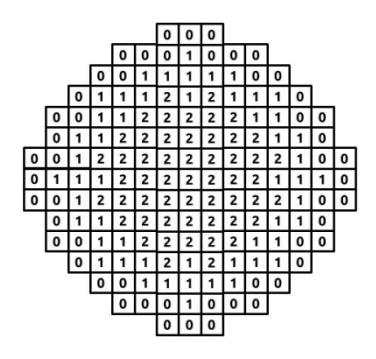
\includegraphics[width=0.75\textwidth]{core_out.in.jpg}
                %\caption{}
            \end{figure}
        \end{column}

        \begin{column}{0.45\textwidth}
            \begin{enumerate}[series=outerlist,topsep=0pt,itemsep=15pt,leftmargin=*,label=(\arabic*)]
                \item[]Innermost fuel discharged
                \item[]Other batches moved to center
                \item[]Fresh fuel always on the end
                \item[]Not used anymore
            \end{enumerate}
        \end{column}

    \end{columns}
\end{frame}


\begin{frame}{In the scatter loading, the core is divided into small regions}
    \begin{columns}

        \begin{column}{0.55\textwidth}
            \begin{figure}
                \centering
                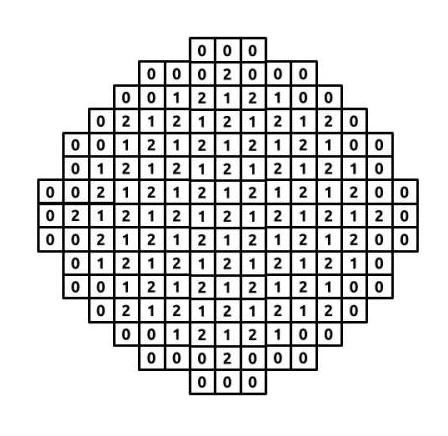
\includegraphics[width=0.75\textwidth]{core_scatter.jpg}
                %\caption{}
            \end{figure}
        \end{column}

        \begin{column}{0.45\textwidth}
            \begin{enumerate}[series=outerlist,topsep=0pt,itemsep=15pt,leftmargin=*,label=(\arabic*)]
                \item[]Assemblies with highest burnup replaced with fresh fuel
                \item[]What advantages does this configuration offer?
            \end{enumerate}
        \end{column}

    \end{columns}
\end{frame}


\begin{frame}{The pressure vessel suffers damage from neutron leakage}
    \begin{enumerate}[series=outerlist,topsep=0pt,itemsep=7pt,leftmargin=*,label=(\arabic*)]
        \item[]Function of power generated and flux shape
        \item[]What shape is angular flux? 
        \item[]Reduce flux without reducing power
        \item[]Placed burned assemblies on the periphery
        \item[]Relocate assemblies from structural critical points
        \item[]Replace some peripheral assemblies with empty ones
        \item[]Add attenuating materials between core and vessel
        \item[]Or add more poisons to peripheral positions
        \item[]Not sure how some of those not reducing power
    \end{enumerate}
\end{frame}


\begin{frame}{The low leakage configuration moves fresh fuel from vessel}
    \begin{columns}

        \begin{column}{0.55\textwidth}
            \begin{figure}
                \centering
                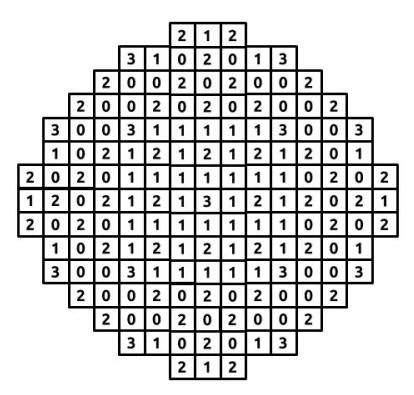
\includegraphics[width=0.75\textwidth]{core_low.leak.jpg}
                %\caption{}
            \end{figure}
        \end{column}

        \begin{column}{0.45\textwidth}
            \begin{enumerate}[series=outerlist,topsep=0pt,itemsep=15pt,leftmargin=*,label=(\arabic*)]
                \item[]Reducing leakage increases burnup
                \item[]Moves peak power closer to center
                \item[]Use of poisons dependent on plant to maintain peak:average
                \item[]Each with different enrichments, on different cycles
            \end{enumerate}
        \end{column}

    \end{columns}
\end{frame}


\begin{frame}[plain]{}
    \centering\LARGE\textbf{Burnup management}
\end{frame}


\addtocounter{framenumber}{-1} 
\begin{frame}{Better fuel utilization will achieve higher burnup}
    \begin{enumerate}[series=blue,topsep=0pt,itemsep=21pt,leftmargin=*,label=(\arabic*)]
        \item[]Switch to the 18, 24 month cycle
        \item[]Requires higher enrichment
        \item[]Reduction in rod worth due to more Pu mass with higher enrichment
        \item[]Pu increases fast:thermal flux
        \item[]Control rods absorb mainly thermal neutrons
    \end{enumerate}
\end{frame}


\begin{frame}{Increased burnup affects structural materials}
    \begin{enumerate}[resume=blue,topsep=0pt,itemsep=21pt,leftmargin=*,label=(\arabic*)]
        \item[]Increased fission gas production
        \item[]More radiation damage from fast neutrons
        \item[]`Increased risk of fuel failure'
        \item[]Though I would question by how much since this isn't happening
    \end{enumerate}
\end{frame}


\begin{frame}{It's not clear what the effect of higher burnup on fuel pools is}
    \begin{enumerate}[series=outerlist,topsep=0pt,itemsep=21pt,leftmargin=*,label=(\arabic*)]
        \item[]Neutron multiplication would be higher per assembly
        \item[]There would be more Pu generated
        \item[]But there would be more fission product poisons too
        \item[]And the fuel would be more fissioned out
        \item[]Obviously, there needs to be an accurate measurement to ensure criticality safety
    \end{enumerate}
\end{frame}


\begin{frame}{Burnup is measured in a variety of ways}
    \begin{enumerate}[series=outerlist,topsep=0pt,itemsep=5pt,leftmargin=*,label=(\arabic*)]
        \item[]Direct measurement -- sensors, fission chambers, flux wires -- during operation
        \item[]Indirect measurement -- after discharge
            \vspace{0.10in}
        \item[]$^{137}Cs$ activity -- $B=a+bA_{Cs}$
        \item[]Directly measures 662 keV gamma
            \vspace{0.10in}
        \item[]Relative measurement --
        \item[]$B=c(e,r)+d(e,r) \cdot \frac{^{134}Cs}{^{137}Cs}$
        \item[]e = enrichment; r = power rating
            \vspace{0.10in}
        \item[]$B=ae^{b\ln{R_0}}$, $R_0=\frac{^{106}Ru\cdot ^{137}Cs}{^{134}Cs^2}$
        \item[]Good for fresh fuel because of short Ru half-life
    \end{enumerate}
\end{frame}


\begin{frame}{\href{https://www.nrc.gov/docs/ML1002/ML100210543.pdf}{NUREG/CR-6998} Table 3.1 burnup confirmation}
    \begin{enumerate}[series=outerlist,topsep=0pt,itemsep=5pt,leftmargin=*,label=(\arabic*)]
        \item[]\textbf{Cs-137 direct measurement}
        \item[]Insensitive to variations in reactor power rating 
        \item[]Requires well defined geometry between detector and assembly
            \vspace{0.10in}
        \item[]\textbf{Cs-134:Cs-137}
        \item[]Insensitive to geometry
        \item[]Short half life, less then 20 y cooling time
        \item[]Dependent on inital enrichment, power rating
            \vspace{0.10in}
        \item[]\textbf{Ru}
        \item[]Insensitive to geometry
        \item[]Less than 9 years cooling time
    \end{enumerate}
\end{frame}


\begin{frame}{Passive neutron measurement can also be used}
    \begin{enumerate}[series=outerlist,topsep=0pt,itemsep=7pt,leftmargin=*,label=(\arabic*)]
        \item[]Cm-244 spontaneous neutron emission dominant source
        \item[]95\% after 10 years
        \item[]92\% after 20 years
        \item[]Uniform signal from all pins
        \item[]Good for safeguards
        \item[]Strong function initial enrichment
        \item[]Geometry sensitive
        \item[]Affected by poisons
    \end{enumerate}
\end{frame}


\begin{frame}[plain]{}
    \centering\LARGE\textbf{Outage management}
\end{frame}


\addtocounter{framenumber}{-1} 
\begin{frame}{Refueling needs to get done as quickly as possible}
    \begin{enumerate}[series=outerlist,topsep=0pt,itemsep=11pt,leftmargin=*,label=(\arabic*)]
        \item[]Lots of activities going on during shutdown
        \item[]Emma Redfoot -- Diablo internship
        \item[]Maintenance and refueling
        \item[]Schedule shutdown during time of low demand
        \item[]Where does the power come from during shutdown?
        \item[]When would be peak demand in Idaho?
    \end{enumerate}
\end{frame}


\begin{frame}{Outages cost a lot of money}
    \begin{enumerate}[series=outerlist,topsep=0pt,itemsep=11pt,leftmargin=*,label=(\arabic*)]
        \item[]Up to \$2 million per day
        \item[]Minimize shutdown period
        \item[]How will \acsp{smr} do it?
        \item[]Then the utility may have to buy replacement power
        \item[]Establish outage organization
        \item[]Inventory of tasks to perform (12,000)
        \item[]Schedule all of the tasks
        \item[]Requires expertise in risk management and decision making
        \item[]\href{https://currently.att.yahoo.com/att/1-200-workers-hired-big-120000470.html}{1,200 workers hired for a big job at Northwest's only nuclear power plant}
    \end{enumerate}
\end{frame}


\begin{frame}{\href{http://www.iaea.org/inis/collection/NCLCollectionStore/_Public/23/014/23014979.pdf}{Outage best practices}}
    \begin{enumerate}[series=outerlist,topsep=0pt,itemsep=11pt,leftmargin=*,label=(\arabic*)]
        \item[]Remove vessel head, prepare fuel handling equipment prior to reloading
        \item[]Assembly, pressure vessel, fuel inspections after unloading
        \item[]In-vessel and ex-vessel equipment repair
        \item[]Reload fuel and close vessel
        \item[]Major equipment inspection and repair (pumps, turbine, etc.)
        \item[]Startup testing
    \end{enumerate}
\end{frame}


\begin{frame}{In addition to refueling, there's lots of \href{http://www-pub.iaea.org/MTCD/Publications/PDF/TRS449_web.pdf}{inspections and testing}}
    \begin{enumerate}[series=outerlist,topsep=0pt,itemsep=15pt,leftmargin=*,label=(\arabic*)]
        \item[]Reactor vessel; Steam generator; Pumps  
        \item[]Turbine and generator; Control rods; Pressurizer
        \item[]Moisture separator; Coolant system; Containment testing
        \item[]Fuel handling system; Instrumentation
        \item[]Diesel generators; Piping; Valves
        \item[]Residual heat removal; Cooling towers
    \end{enumerate}
\end{frame}


%\begin{frame}{}
%    \begin{equation}
%        \LARGE
%    \end{equation}
%
%    \begin{equation}
%        \LARGE
%    \end{equation}
%
%    \vspace*{\fill}
%
%    \begin{enumerate}[series=outerlist,topsep=0pt,itemsep=21pt,leftmargin=*,label=(\arabic*)]
%    \end{enumerate}
%
%    \vspace*{\fill}
%
%    \begin{equation}
%        \LARGE
%    \end{equation}
%
%    \vspace*{\fill}
%
%    \begin{enumerate}[series=outerlist,topsep=0pt,itemsep=21pt,leftmargin=*,label=(\arabic*)]
%    \end{enumerate}
%\end{frame}


%\begin{frame}{}
%    \begin{enumerate}[series=outerlist,topsep=0pt,itemsep=21pt,leftmargin=*,label=(\arabic*)]
%    \end{enumerate}
%
%    \vspace*{\fill}
%
%    \begin{equation}
%        \LARGE
%    \end{equation}
%
%    \vspace*{\fill}
%
%    \begin{enumerate}[series=outerlist,topsep=0pt,itemsep=11pt,leftmargin=*,label=(\arabic*)]
%    \end{enumerate}
%
%    \vspace*{\fill}
%
%    \begin{equation}
%        \LARGE
%    \end{equation}
%\end{frame}


%\begin{frame}{}
%    \begin{figure}
%        \centering
%        \includegraphics[width=0.85\textwidth]{}
%%       \caption{}
%    \end{figure}
%\end{frame}


\begin{frame}[plain]{}
    \begin{figure}
        \centering
        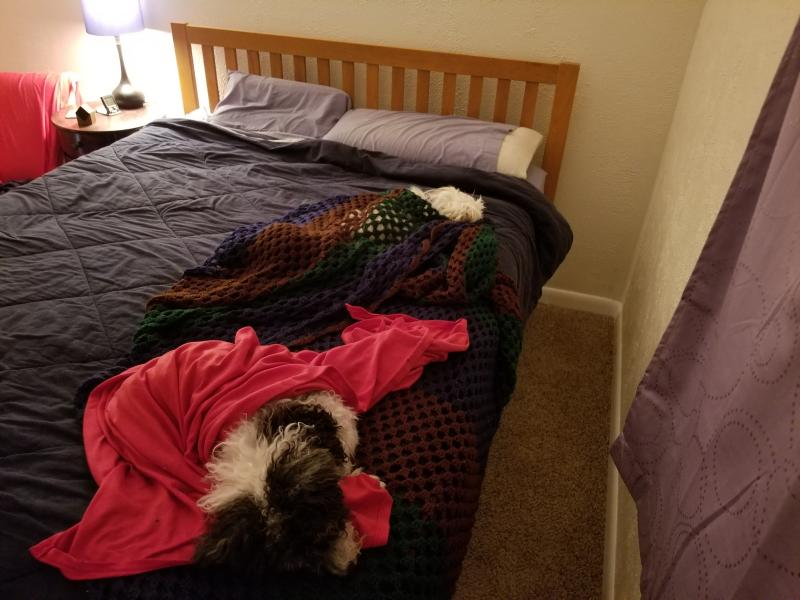
\includegraphics[width=0.75\textwidth]{final.jpg}
%        \caption{}
    \end{figure}
\end{frame}


%%%%%%%
%\begin{frame}{}
%    \begin{columns}
%
%        \begin{column}{0.50\textwidth}
%            \begin{enumerate}[series=outerlist,topsep=0pt,itemsep=21pt,leftmargin=*,label=(\arabic*)]
%                \item[]
%                \item[]
%            \end{enumerate}
%        \end{column}
%
%        \begin{column}{0.50\textwidth}
%            \begin{enumerate}[series=outerlist,topsep=0pt,itemsep=21pt,leftmargin=*,label=(\arabic*)]
%                \item[]
%                \item[]
%            \end{enumerate}
%        \end{column}
%
%    \end{columns}
%\end{frame}

%    \begin{figure}
%        \centering
%        \includegraphics[width=0.75\textwidth]{wsc.png}
%        \caption{\acs{wsc}}
%    \end{figure}


%\begin{frame}{References}
%    \bibliographystyle{nsf}
%    \footnotesize
%    \bibliography{references}
%\end{frame}
%%%%%%%


\end{document}
